\documentclass[12pt]{article}
\usepackage{times}
\usepackage{titling}
\usepackage{graphicx}

% modify the font size of title, author and date
\pretitle{\begin{center}\bf \Large} \posttitle{\par\end{center}}
\preauthor{\begin{center}
            \small \small \lineskip 0.5em%
            \begin{tabular}[t]{c}}
\postauthor{\end{tabular}\par\end{center}}
\predate{\begin{center}\small} \postdate{\par\end{center}}

\bibliographystyle{IEEEtran}

% ====================================================================

\title{ECE 552: Computational Techniques for \\Circuit Analysis - Fall 2010\\
Project Report}
\author{Zigang Xiao}
\date{\today}
\begin{document}
\maketitle

\section{Introduction}
\subsection{Project description}
In this project, a circuit simulator program is implemented.
It can read SPICE like input netlist and perform three types of 
analysis, namely I)~DC analysis, II)~AC analysis and III)~Transient analysis.

\subsection{Description of Algorithms}
The program accepts an input netlist file and outputs node voltages and branche
currents.  The information of nets, nodes and initial guess values will be read
from the input file accordingly.  Moreover, control parameters such as
begining, ending frequency and step size of AC analysis, finishing time and
time step of transient analysis and the name of node that needs to be plot will
be saved. The program determines which kind of analysis to be performed
according to the input, and perform the analysis.  Following are the details
for three types of analysis.

\subsubsection{DC Analysis}
Among the three types of analysis, DC analysis is the most important one since 
it will be used to determine the DC operating point for both AC analysis and
transient analysis.
If the nets are all linear devices, a MNA matrix will be built and solved.
If there are non-linear devices, they will be lineared and 
Newton-Raphson iteration will be applied to iteratively solve for the node
voltages. To overcome convergence issue, damped Newton-Raphson iteration is implemented.
Note that capacitors and inductors are treated as open-circuited and short-circuited
in DC analysis.

\subsubsection{AC Analysis}
In AC analysis, the DC operating point of the circuits will be obtained first, 
using the DC analysis. AC voltage source are treated as short-circuited.
Given a frequency value $f$, capacitors, inductors, diode and BJT are stamped 
according to $f$.
The voltages of the nodes to be plot will be acquired and output to a file.

\subsubsection{Transient Analysis}
Similar to AC analysis, DC analysis will be performed first to obtain 
the initial value at time $t=0$.
Then, Newton-Raphson iteration will be used to solve for node voltages
for each successive time step. 
Backward Euler integration method and the Norton equivalent model 
is used in the project, since they will not introduce extra voltage sources.
Furthermore, Backward Euler method is more accurate than Forward Euler 
and much simpler than Trapezoidal method.

\subsection{Implementation Details}
The program is implemented in C++. The nets and nodes are encapsulated as classes,
where different devices can be modeled as subclasses of nets.
C++ Standard Template Library is utilized in the program.

UMFPACK~\cite{umfpack} is used 
to solve sparse matrix that contains complex number entries.
Compressed row/column index storage method for sparse matrix is hard for human to read and
operate on.  UMFPACK supports a much simpler representation, i.e.,
Triplet arrays. Each element in the array is represented as a triplet $(i,j,v)$, 
where $[i,j]$ is the index and $v$ is the value.
Duplicate index entry can exist in the array. UMFPACK provides a 
handy function that can help us transform the triplet form to the column index form.
Hence, when stamping an element, we can simply add a triplet to the arrays.
By using this method, the \texttt{large.txt} test case can be solved 
at around 0.01 second when run on a Intel Core II Duo 2.4 GHz machine.

During the implementation, the convergence issue occurs.
Damped Newton-Raphson method must be used. The dampen value is set to 0.1.

Note that besides the circuit nodes, voltage source, vccs, cccs and ccvs 
will introduce extra rows and columns in the MNA matrix.
Their index is stored in STL map class for $O(1)$ access.
Note that in my implementation, ground node is assigned a row and a column 
in the matrix for convenient. The triplet will not be inserted whenever 
$i=0$ or $j=0$.  Otherwise the MNA matrix will become singular.
The matrix right hand side (RHS) will be set to 0 before solving.

% ====================================================================
\section{Equations used in Analysis}
\subsection{DC Analysis}
\subsection{AC Analysis}
\subsection{Transient Analysis}

% ====================================================================

\section{Experimental Results}
\subsection{Results of Phase I (Linear DC Analysis)}
Table~\ref{tab:phase1} in page~\pageref{tab:phase1} gives the output of phase I.


% --------------------------------------------------------------------

\subsection{Results of Phase II (Nonlinear DC Analysis)}
Table~\ref{tab:phase2} in page~\pageref{tab:phase2} gives the output of phase II.

% --------------------------------------------------------------------

\subsection{Results of Phase III (AC Analysis and Transient Analysis)}
\subsubsection{bjt.txt}
Figure~\ref{fig:bjt} shows the result of bjt.txt.

\begin{figure}[htbp]
  \centering
    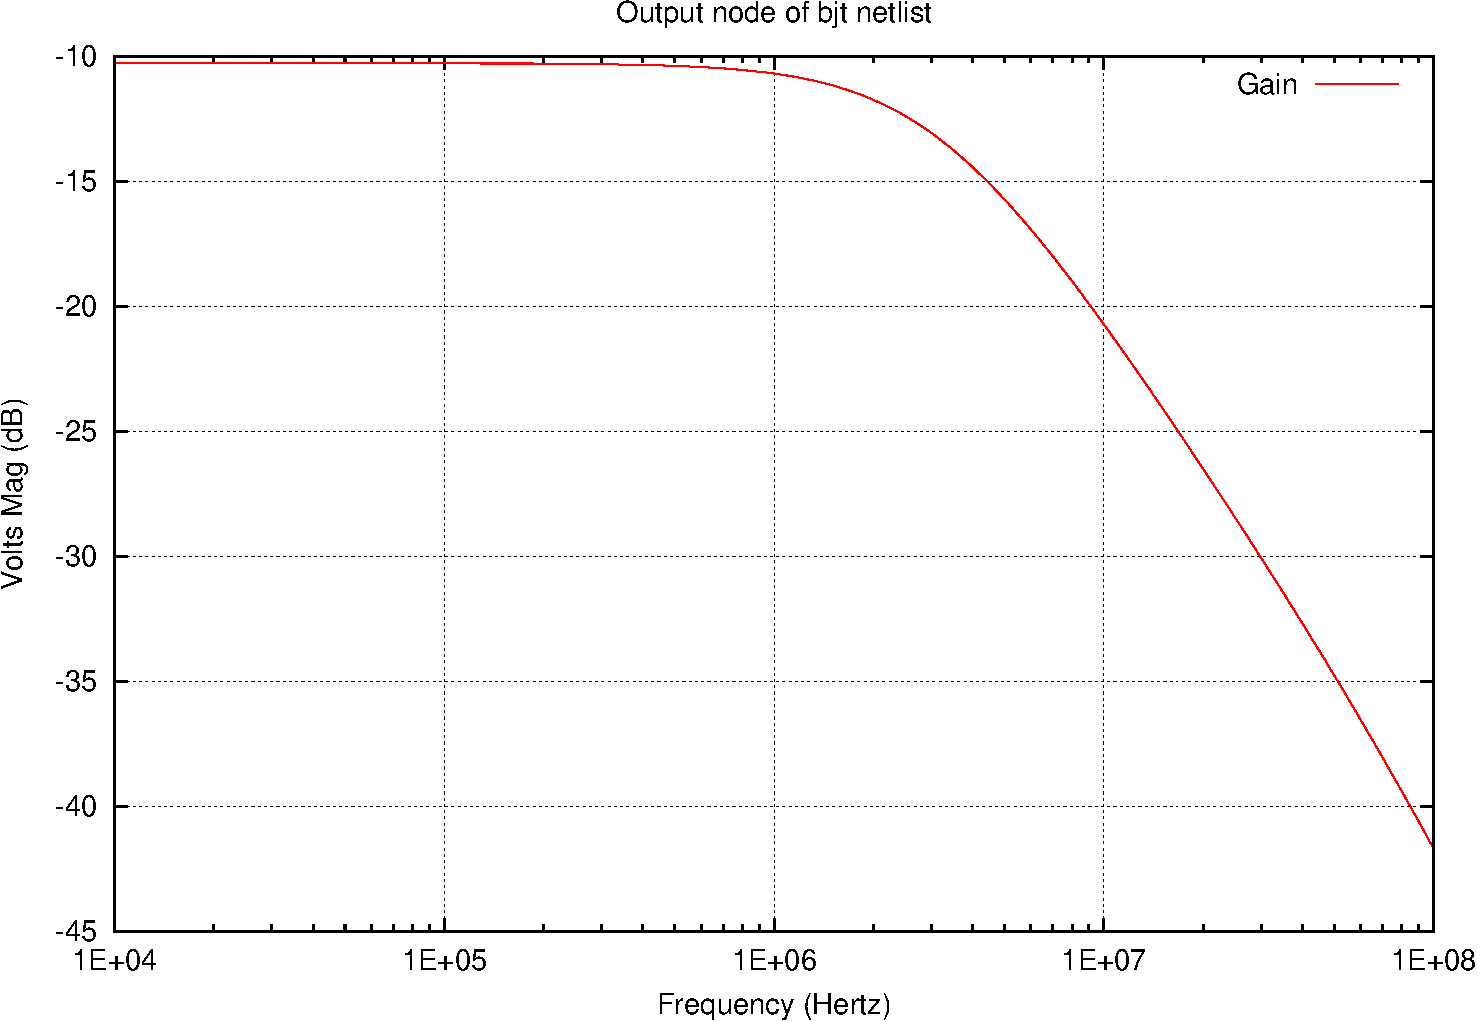
\includegraphics[width=.8\textwidth]{bjt_out_g-crop.pdf}

    \vspace{2em}

    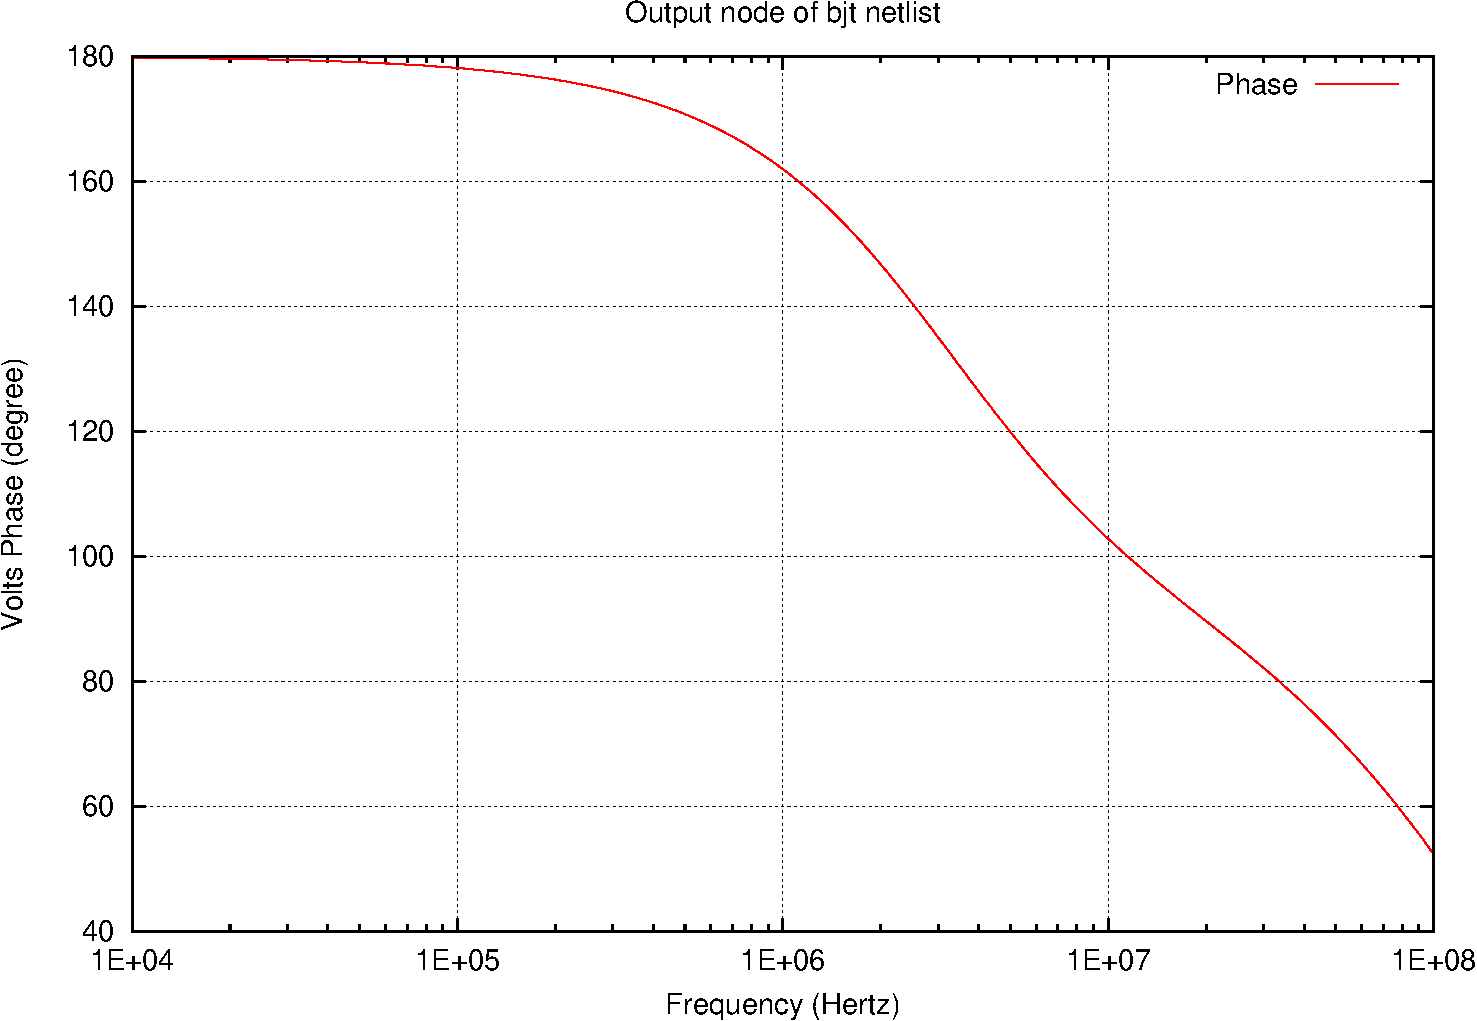
\includegraphics[width=.8\textwidth]{bjt_out_p-crop.pdf}
  \caption{Gain and phase plot of node `out'.}
  \label{fig:bjt}
\end{figure}


\subsubsection{741\_amplifier.txt}
Figure~\ref{fig:741} shows the result of 741\_amplifier.txt.

\begin{figure}[htbp]
  \centering
    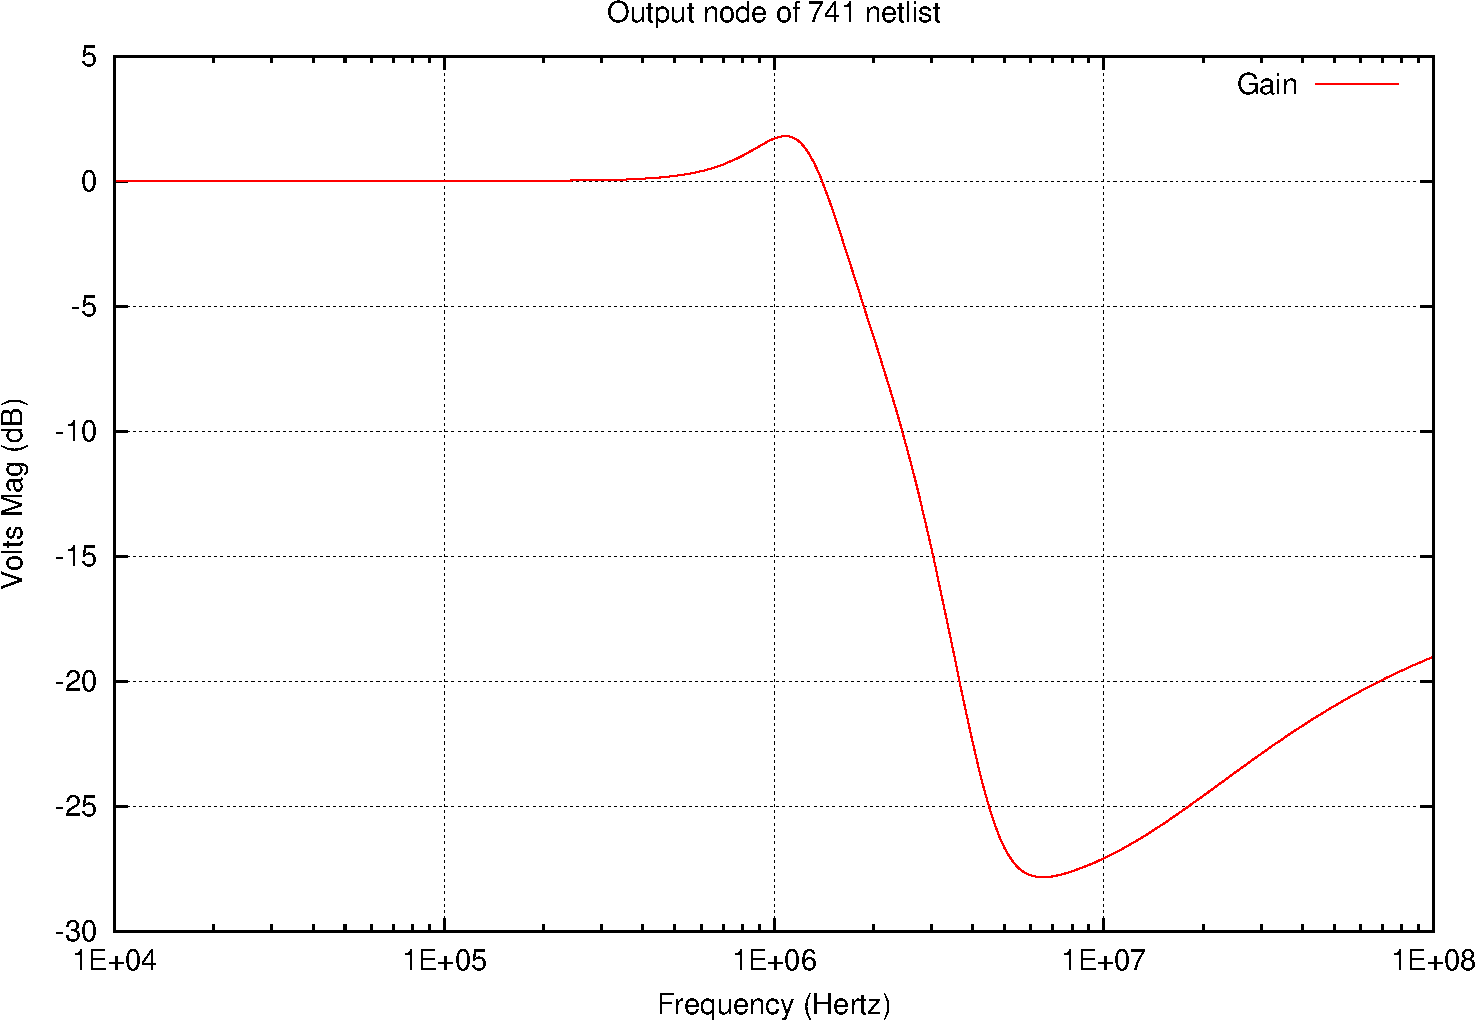
\includegraphics[width=.8\textwidth]{741_amplifier_22_g-crop.pdf}

    \vspace{2em}

    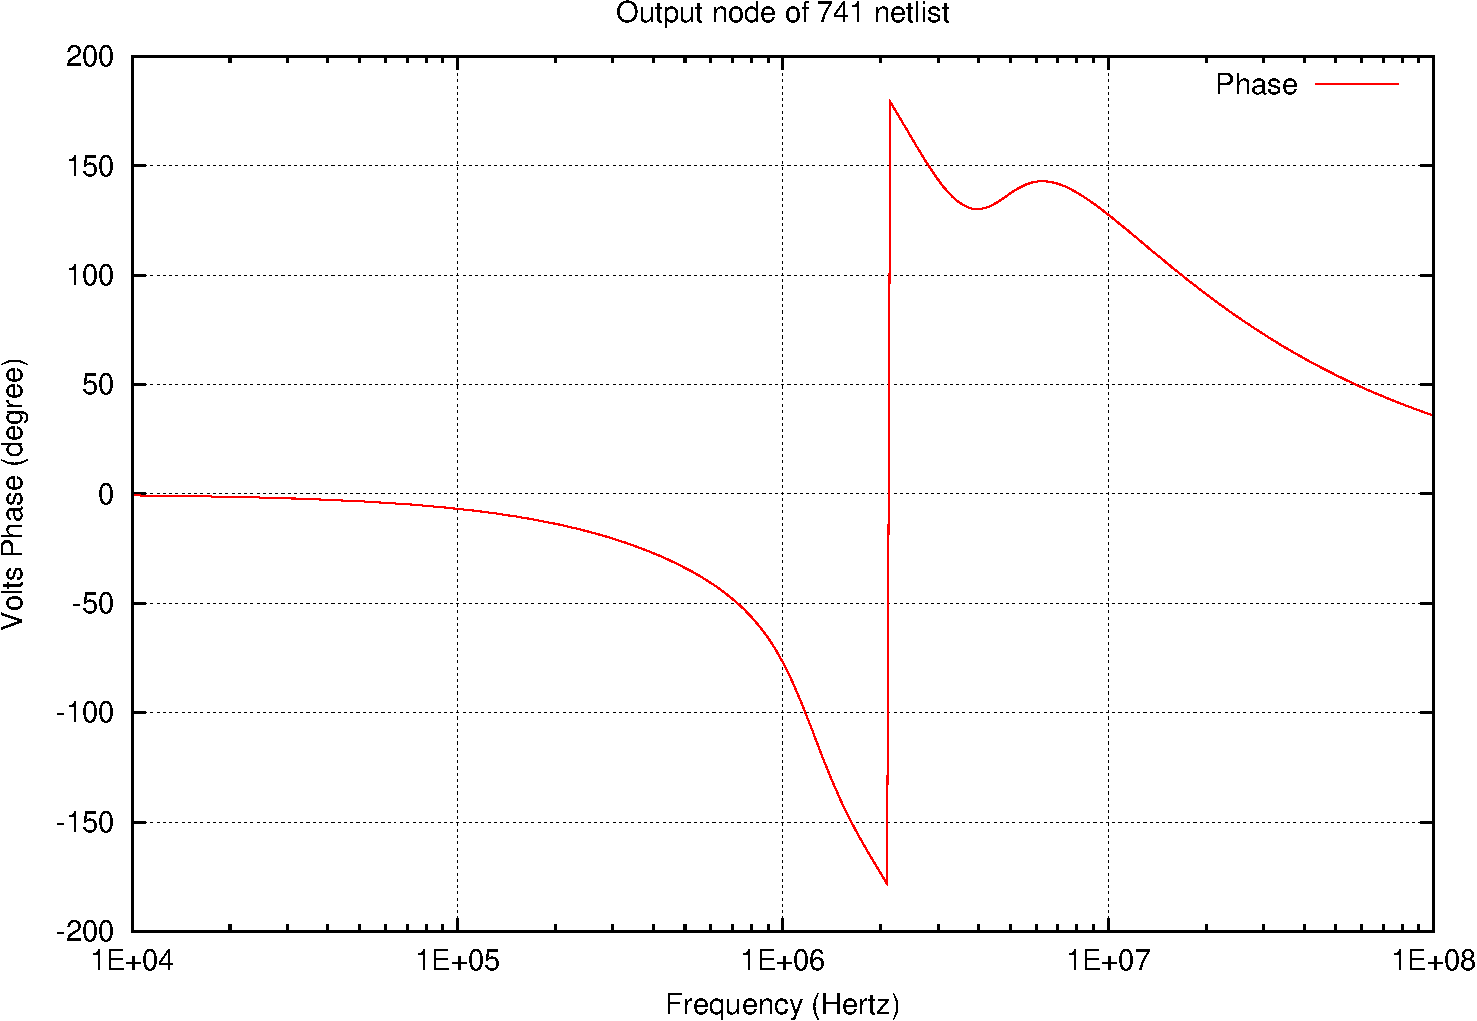
\includegraphics[width=.8\textwidth]{741_amplifier_22_p-crop.pdf}
  \caption{Gain and phase plot of node `22'.}
  \label{fig:741}
\end{figure}

\subsubsection{amp\_tran1.txt}
Figure~\ref{fig:tran} shows the result of amp\_tran1.txt.

\begin{figure}[!htbp]
  \centering
    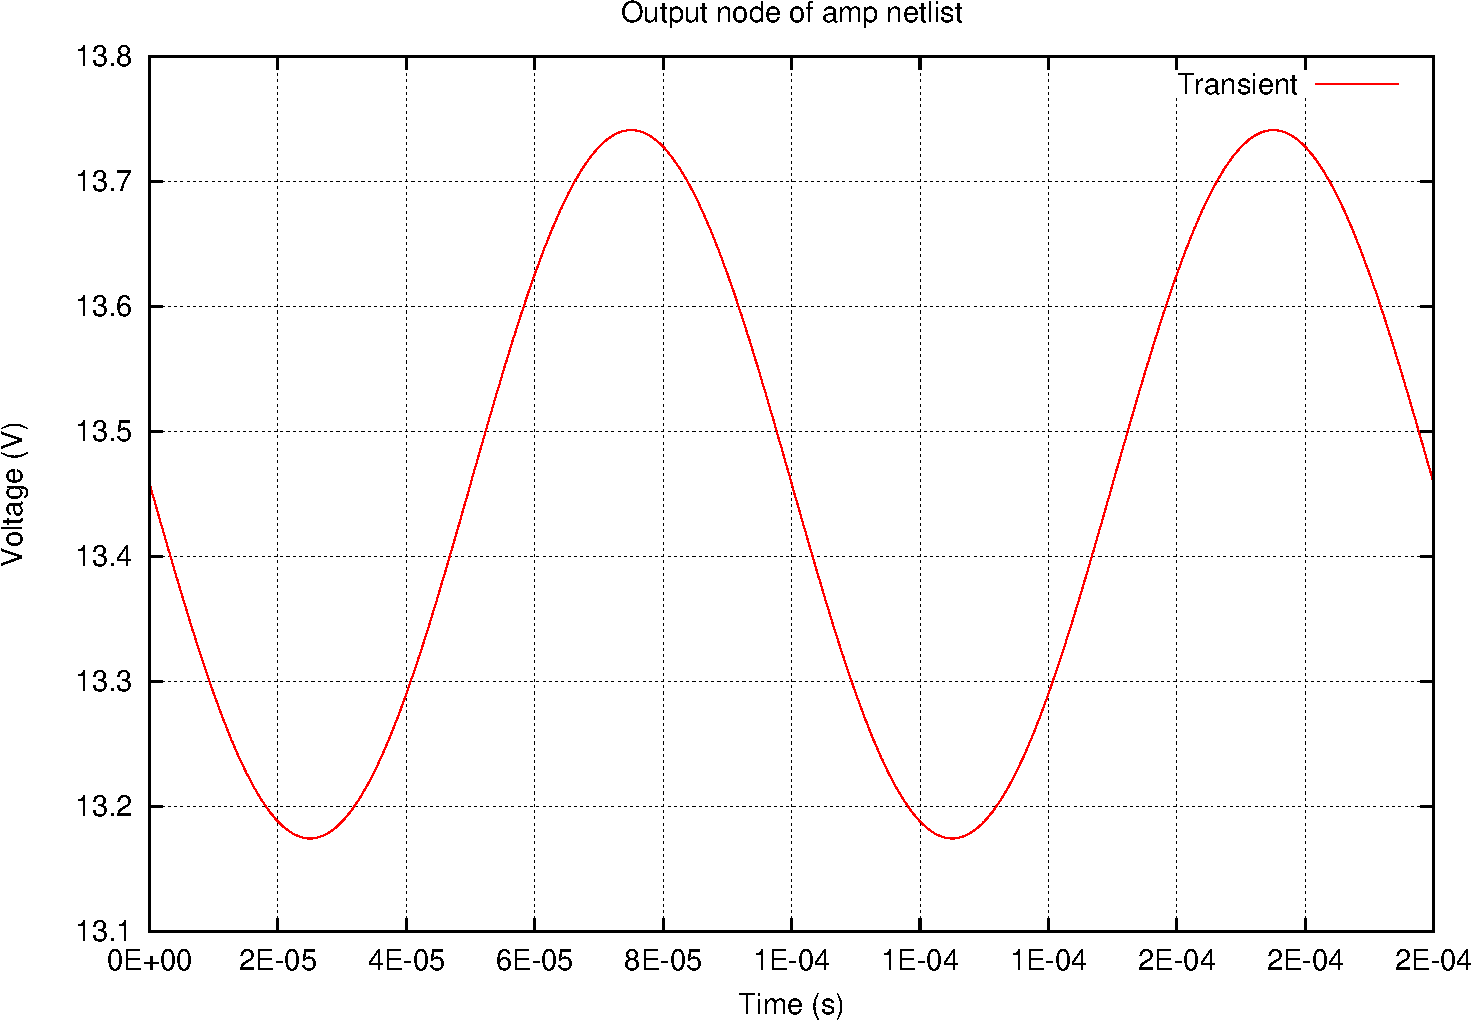
\includegraphics[width=.8\textwidth]{amp_tran1_out1_t-crop.pdf}

    \vspace{2em}

    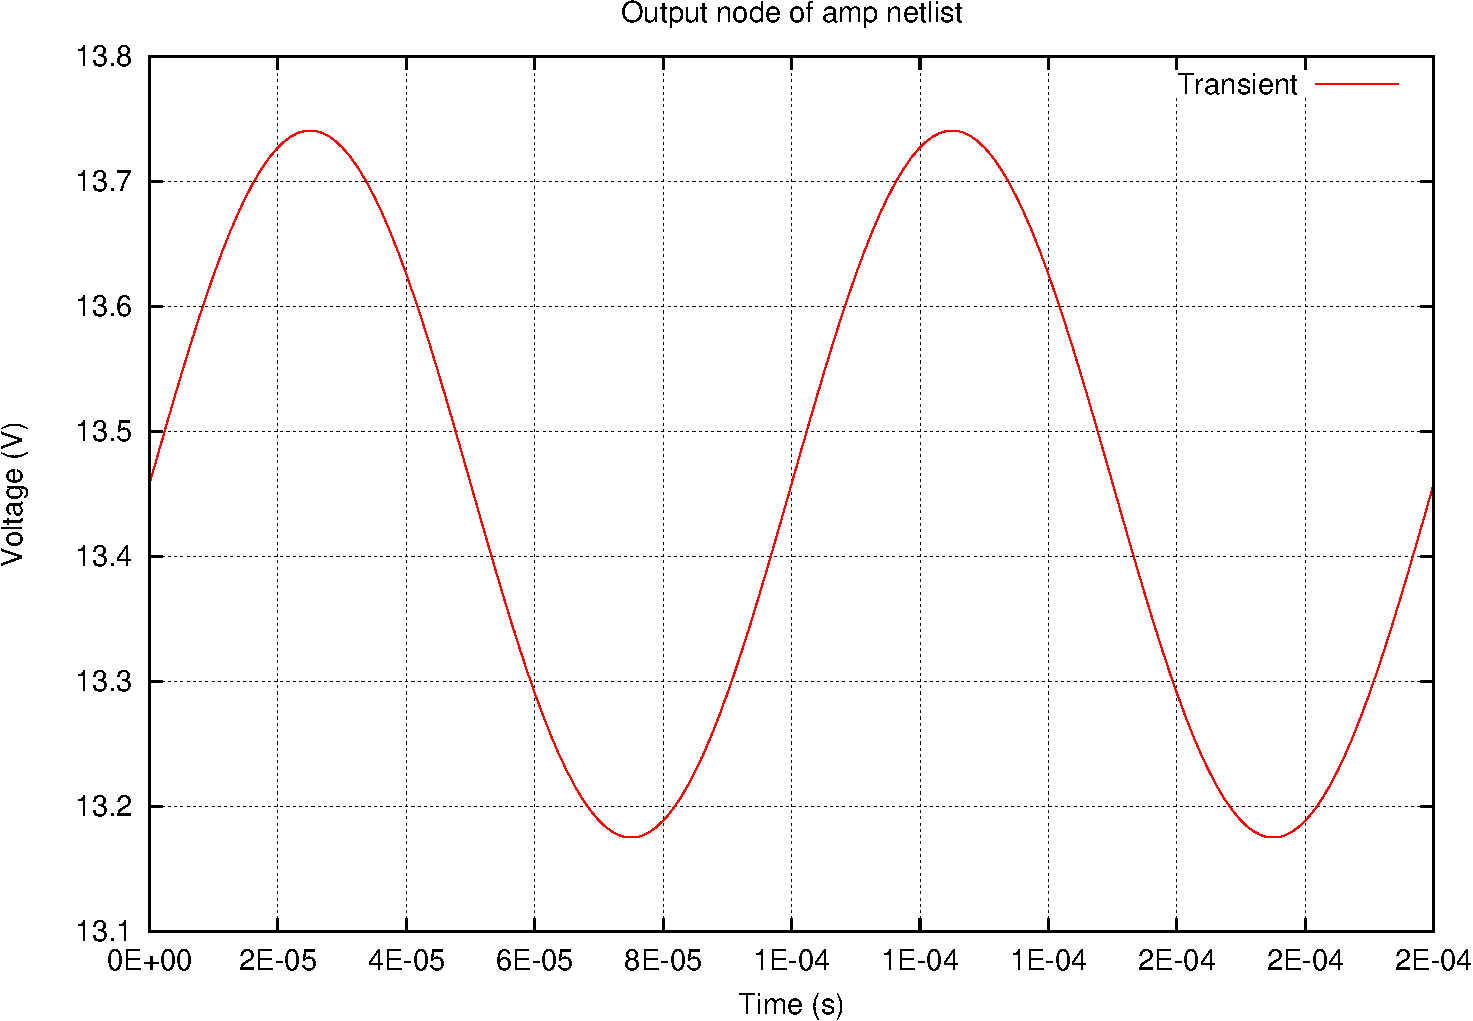
\includegraphics[width=.8\textwidth]{amp_tran1_out2_t-crop.pdf}
  \caption{Voltage plot of node `out1' and `out2'.}
  \label{fig:tran}
\end{figure}



\begin{table}[h]
  \centering
\begin{tabular}{|p{\linewidth}|}
\hline
\scriptsize
\begin{verbatim}
* representative
voltage at node a = 1.000000e+00
voltage at node b = 6.000000e-01
voltage at node c = 1.600000e+00
voltage at node d = 1.701538e+01
voltage at node e = -3.040000e+01
voltage at node f = -1.600000e+01
voltage at node g = -2.200000e+00
voltage at node h = -1.075513e+03
current throught source v1 = -2.000000e-01
current throught source e1 = 2.569231e+00
current throught source h1 = 8.962609e+01
current throught source f1 = -1.600000e+00

* large
run-time: 0.01593
machine clock frequency: 2.26 GHz Intel Core 2 Duo
voltage at node 1 = 1.999980e-10
voltage at node 2 = 5.999940e-10
voltage at node 3 = 1.199988e-09
voltage at node 4 = 1.999980e-09
voltage at node 5 = 2.999970e-09
voltage at node 6 = 4.199958e-09
voltage at node 7 = 5.599944e-09
voltage at node 8 = 7.199928e-09
voltage at node 9 = 8.999910e-09
voltage at node 10 = 1.099989e-08
voltage at node 11 = 1.319987e-08
voltage at node 12 = 1.559984e-08
voltage at node 13 = 1.819982e-08
voltage at node 14 = 2.099979e-08
voltage at node 15 = 2.399976e-08
voltage at node 16 = 2.719973e-08
voltage at node 17 = 3.059970e-08
voltage at node 18 = 3.419966e-08
voltage at node 19 = 3.799962e-08
voltage at node 20 = 4.199958e-08

* error
Error: dependent voltage source [v2] of cccs [f1] not present!
Error: dependent voltage source [v3] of ccvs [h1] not present!
\end{verbatim}\\
\hline
\end{tabular}
  \caption{Phase I output.}
  \label{tab:phase1}
\end{table}

\begin{table}[h]
  \centering
\begin{tabular}{|p{\linewidth}|}
\hline
\scriptsize
\begin{verbatim}
* Diode:

Iteration begins:
iteration: 1, difference = 3.287877e-03
iteration: 2, difference = 1.884439e-04
iteration: 3, difference = 6.766938e-07
iteration: 4, difference = 8.683831e-12
Total number of iterations: 4

Result:
voltage at       0 = 0.000000e+00
voltage at       1 = 2.000000e+00
voltage at       2 = 7.030988e-01
current throught source v1 = -6.484506e-04

* BJT:

Iteration begins:
iteration: 1, difference = 9.000161e-01
iteration: 2, difference = 6.440751e-04
iteration: 3, difference = 8.155846e-06
iteration: 4, difference = 1.286492e-09
iteration: 5, difference = 9.566619e-16
Total number of iterations: 5

Result:
voltage at       0 = 0.000000e+00
voltage at  supply = 5.000000e+00
voltage at   cbias = 4.286034e+00
voltage at     out = 9.198898e-02
voltage at       b = 7.161394e-01
voltage at  input2 = 9.000000e-01
voltage at  input1 = 9.000000e-01
current throught source vcc = -2.021662e-03
current throught source vin = -1.838606e-05
current throught source vin2 = -1.838606e-05
\end{verbatim}\\
\hline
\end{tabular}
  \caption{Phase II output.}
  \label{tab:phase2}
\end{table}



\bibliography{552report}
\end{document}
